
\section{Implementation}

This section will detail specific implementation details about the application created.

\subsection{API}

The API was written using the FastAPI\footnote{\url{https://fastapi.tiangolo.com/} (Accessed 09/05/2023)} framework due to its simple syntax, built-in support for data validation and serialisation, and its support for OpenAPI documentation that allows developers to easily write documentation and have it hosted to allow users to explore the API.
The use of OAuth2 with JSON Web Tokens meant the API endpoints are secure and only usable by registered users, which allows for the safe, public hosting of this API.

\subsection{Data Storage}

This application will create a local SQLite\footnote{\url{https://sqlite.org/index.html} (Accessed 09/05/2023)} database that will be interacted with using the object relational mapping library SQLAlchemy\footnote{\url{https://www.sqlalchemy.org/} (Accessed 09/05/2023)}. The following tables will be created:

\begin{itemize}[noitemsep]
    \item \textbf{wakeable\_devices} These are the IP-based devices that can be woken over the network by sending a magic packet to them.
    \item \textbf{schedules} These relate a device to many recurring points in time at which the device should be woken up by the application. Each schedule can be toggled individually.
    \item \textbf{watcher\_devices} These are devices that can be searched for locally using the methods described in Section~\ref{subsec:services}. Each device will have a timeout that allows users to restrict how often a detection of this device triggers devices to wake up.
    \item \textbf{watcher\_wakeable\_mapping} This table shows the many-to-many associations between wakeable and watcher devices. Each mapping also stores which mediums should be watched; for example, should the application look for it using Bluetooth.
    \item \textbf{users} This will store the user information to help secure this API. This application will only consider a single admin user.
    \item \textbf{services} Stores information about the background services a user can run and whether they should be run on application startup. The services available are detailed in Section~\ref{subsec:services} and each can be toggled on or off at any point.
    \item \textbf{environment\_listeners} Stores information about each environment listener including what it is watching (noise, light, or temperature), what the threshold value is (to determine when to wake the device), whether this threshold is an upper/lower limit and a reference to the device being woken. 
\end{itemize}

\subsection{Other Details}

\vspace{2mm}
\subsubsection{Docker}

For easy setup, a Dockerfile is provided to allow a user to start the application with a single command without having to manually install any of the dependencies.

\vspace{2mm}
\subsubsection{Environmental Sensing}

The Enviro\footnote{\url{https://shop.pimoroni.com/products/enviro?variant=31155658489939} (Accessed 10/05/2023)} kit and the corresponding Python library\footnote{\url{https://github.com/pimoroni/enviroplus-python} (Accessed 10/05/2023)} was used in conjunction with a Raspberry Pi 4 to detect various environmental factors. 

\subsection{Application Diagram}

Figure~\ref{fig:app-architecture} shows a breakdown of the application architecture. To help improve the maintainability, the applications is broken down into different layers that are abstract from each other, such that any of them could easily be replaced.

\begin{figure}[ht]
    \centering
    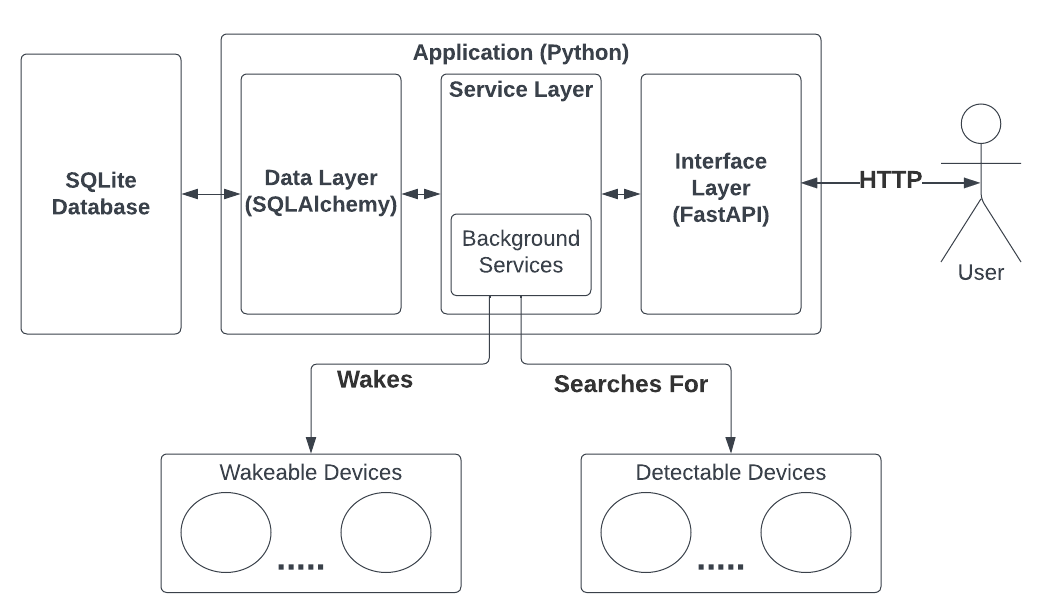
\includegraphics[width=\columnwidth]{assets/application.png}
    \caption{A diagram showing the application architecture.}
    \label{fig:app-architecture}
\end{figure}